% https://tex.stackexchange.com/a/761264/322482
\documentclass[tikz,border=5pt]{standalone}
\usetikzlibrary{ext.paths.ortho}
\begin{document}

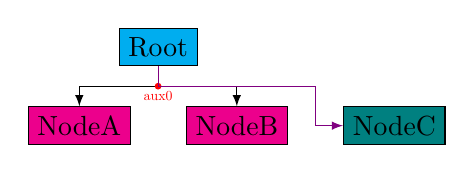
\begin{tikzpicture}[>=latex]
\node[draw,fill=cyan] (Root) {Root};

\node[draw,fill=magenta] at (-1,-1) (nodeA) {NodeA};
\node[draw,fill=magenta] at (1,-1) (nodeB) {NodeB};
\node[draw,fill=teal] at (3,-1) (nodeC) {NodeC};
\draw[->] (Root) |-| (nodeA);
\draw[->] (Root) |-| (nodeB) coordinate[pos=0.25] (aux0);

\filldraw[red] (aux0) circle[radius=1pt] node[below,scale=.5] {aux0};

\draw[->,violet] (Root) |- (aux0) -|-[ratio=.85] (nodeC);

\end{tikzpicture}
\end{document}